% EclipseFP-JE.tex
\begin{hcarentry}[updated]{EclipseFP}
\report{JP Moresmau}%11/14
\status{stable, maintained, and actively developed}
\participants{building on code from Alejandro Serrano Mena, Thomas ten Cate, B.\ Scott Michel, Thiago Arrais, Leif Frenzel, Martijn Schrage, Adam Foltzer and others}
\makeheader

%**<img width=500 src="./eclipsefp-screenshot2.jpg">
%*ignore
\begin{center}
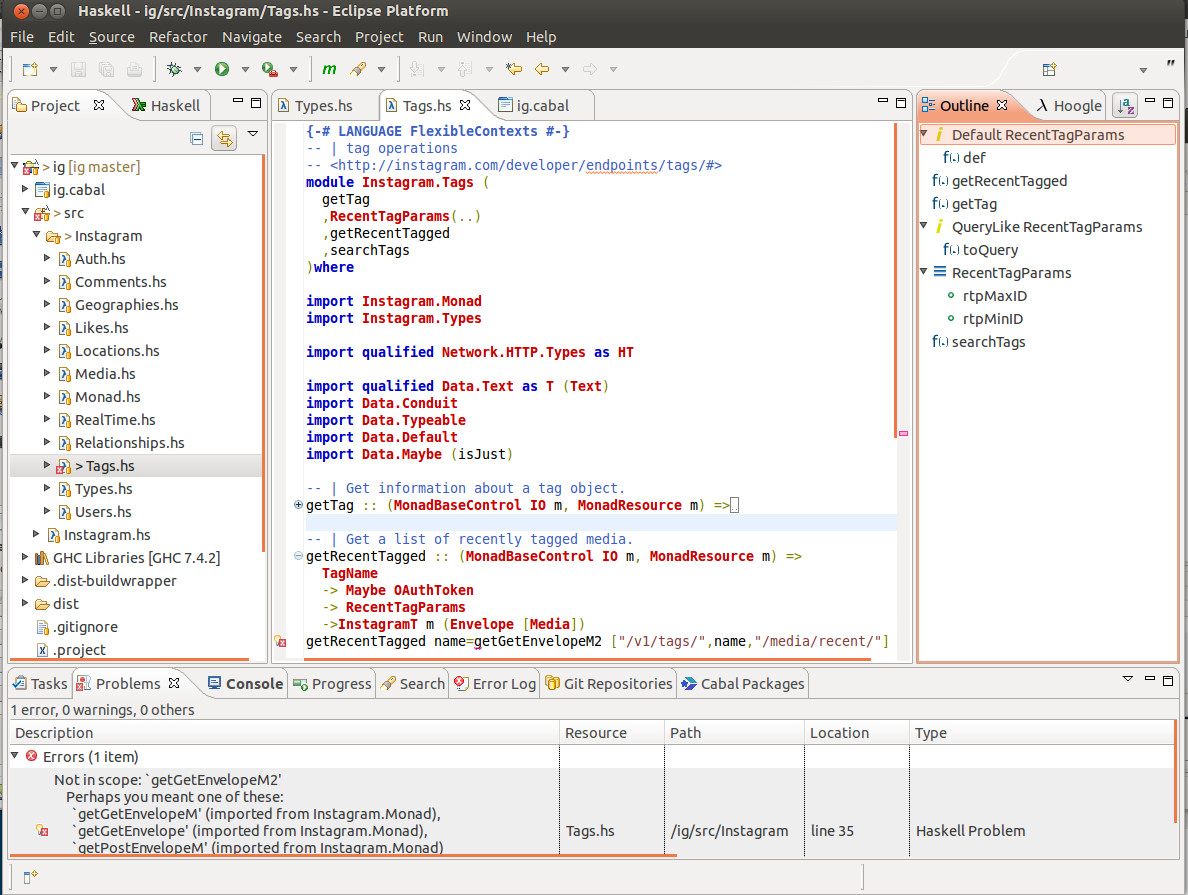
\includegraphics[width=0.47\textwidth]{html/eclipsefp-screenshot2.jpg}
\end{center}
%*endignore

EclipseFP is a set of Eclipse plugins to allow working on Haskell code
projects. Its goal is to offer a fully featured Haskell IDE in a platform
developers coming from other languages may already be familiar with. It
provides the following features, among others:

\begin{description}
  \item[Cabal Integration] \hfill \\ Provides a .cabal file editor, uses Cabal
    settings for compilation, allows the user to install Cabal packages from
    within the IDE. Supports cabal sandboxes (or cabal-dev) to provide install isolation and project
    dependencies inside an Eclipse workspace.  \item[GHC Integration] \hfill
    \\ Compilation is done via the GHC API, syntax coloring uses the GHC
  Lexer.  \item[Productive Coding] \hfill \\ Quick fixes for common errors,
    warnings, and HLint suggestions. Automatic organization of imports.
    Autocompletion. Find and rename across modules and projects.
    Stylish-haskell integration for consistent code formatting.
  \item[Live Programming] \hfill \\ A Haskell worksheet allows the developer to see
    values of expressions, including images and HTML content, as the code changes.
  \item[Debugging] \hfill \\ Easy to launch GHCi sessions on any module with
    proper parameters. Manages breakpoints, the evaluation of variables and
    expressions uses the Eclipse debugging framework, and requires no
    knowledge of GHCi syntax. Also integrates with Yesod (launch the web
    application from EclipseFP). Running a program with profiling options
    results in profiling graphs being displayed in the UI for easy analysis.
  \item[Browsing] \hfill \\ The Haskell Browser perspective allows the user to
    navigate the list of packages and their documentation. It integrates
    seamlessly with Hackage. The Haskell module editor provides code folding,
    outline view of the module, popup of types and documentation mouse hovers,
    etc.  \item[Testing] \hfill \\ EclipseFP integrates with Haskell test
      frameworks, most notably HTF, to provide UI feedback on test failures.
\end{description}

The source code is fully open source (Eclipse License) on github and anyone
can contribute. Current version is 2.6.1, released in July 2014, and more
versions with additional features are planned and actively worked on. Feedback
on what is needed is welcome! The website has information on downloading
binary releases and getting a copy of the source code. Support and bug
tracking is handled through Sourceforge forums and github issues. We welcome
contributors!

\FurtherReading
\begin{compactitem}
\item \url{http://eclipsefp.github.com/}
\item \url{http://jpmoresmau.blogspot.com/}
\end{compactitem}
\end{hcarentry}
